\documentclass[11pt,a4paper]{article}
\usepackage{amsmath,amssymb}
\usepackage{graphicx}
\usepackage{setspace}
\usepackage{tikz}
\usepackage[margin=1in]{geometry}
\usepackage{booktabs}
\usepackage{multirow}
\usepackage[numbers]{natbib}
\usepackage{natbib}
\usepackage{parskip}
\usepackage{float}
\usepackage{tablefootnote}
\usepackage[linesnumbered,ruled,vlined]{algorithm2e}
\providecommand{\keywordname}{\textbf{Keywords:}} % Customize how "Keywords:" appears
\newcommand{\keywords}[1]{%
  \par\addvspace{\baselineskip}% Adds some space above the keywords
  \noindent\keywordname\enspace\ignorespaces#1 % Displays "Keywords:" followed by the actual keywords
}
\newcommand{\citeboth}[1]{\citeauthor{#1} \citep{#1}}

% Define a command to create a hyperlink with only the figure number
\newcommand{\figref}[1]{%
    \hyperref[fig:#1]{Figure \ref{fig:#1}}%
}

% Define a command to create a hyperlink with only the algorithm number
\newcommand{\algoref}[1]{%
    \hyperref[alg:#1]{Algorithm \ref{alg:#1}}%
}

\usepackage[
    colorlinks=true,      
    linkcolor=red,       
    citecolor=blue,       
    urlcolor=blue,        
]{hyperref}


\title{Investigating the Impact of Macroeconomic Indicators

on the FTSE 250 Index Using Statistical and Machine Learning Methods}
\author{Mateen Khan}
\date{\today}

\begin{document}

\maketitle

\begin{abstract}
    This study investigates the impact of the Consumer Price Index (CPI), Bank of England Base Rate, US Dollar (USD) and British Pound Sterling (GBP) exchange rate, and the money supply (M3) measure on the price of the FTSE 250 Index (FTSE250).
    In addition, it assesses the effectiveness of radial basis function neural networks (RBFNN) as a tool to forecast the price of the FTSE 250 Index based on the same set of macroeconomic variables. This study finds quantitative estimates for the short-term and long-term impacts of the aforementioned macroeconomic indicators on the price of the FTSE 250 Index. It also demonstrates the effectiveness of radial basis function neural networks as a short-term forecasting tool for the price of the FTSE 250 Index.
    \keywords{macroeconomic indicators, FTSE 250, autoregressive distributed lag model, radial basis function neural network, time-series forecasting}
\end{abstract}

\section{Introduction}

The stock market is a significant component of the financial system and 
plays a crucial role in the broader economy. Consequently, economic policy 
makers take the stock market into account when making fiscal policy 
decisions using a combination of quantitative and qualitative methods. 
These methods such as econometric modelling and forecasting, and empirical 
analysis allow them to understand the short-term and long-term effects of 
macroeconomic indicators
on the wider economy through the stock market (\citeboth{DemirgucKunt1996}).

Macroeconomic indicators can also be effectively used in machine learning 
methods to forecast stock prices by serving as input features that capture 
the economic environment’s influence on stock market behaviour. By carefully 
selecting the most relevant indicators, 
as well as choosing the appropriate models, machine learning can enhance the accuracy of stock price forecasts (\citeboth{Prasad2023}).

The significance of this study is to quantify the effects of macroeconomic indicators on the stock market as well as assessing the use of these indicators to forecast stock market prices over the short-term and long-term. In addition, the study seeks to understand which macroeconomic indicators are most relevant in capturing the dynamics of a stock market to aid forecasting.

In particular, the objectives of this study are to address how specific macroeconomic indicators influence stock market prices in a developed economy, and whether machine learning models can substitute traditional econometric models in predicting stock market prices. It aims to:
\begin{enumerate}
    \item examine the short-term and long-term effects of macroeconomic indicators on the price of the FTSE250
    \item investigate whether machine learning techniques can provide accurate short-term and long-term forecasts of the price of the FTSE250 when using a small dataset.
\end{enumerate}

In order to analyse the dynamic relationship between the variables in the time series data, this study
will employ the Autoregressive Distributed Lag (ARDL) model in conjunction with an Error
Correction Model (ECM). This research also employs a radial basis function neural network to predict the price movements of the FTSE250.

The remainder of this paper will be organised as follows. 
Section \ref{sec:lit} provides a brief review of the literature in this problem space and explains the rationale behind the selection of macroeconomic variables.
Section \ref{sec:meth} presents the methodology. Section \ref{sec: results} discusses the results and Section \ref{sec: conc} concludes
the study.

\section{Literature Review}
\label{sec:lit}

\subsection{Stock Market-Macroeconomic Relationships}

The findings of \citeboth{ChenRollRoss1986} state that a long-term equilibrium relationship 
exists between stock market prices and relevant macroeconomic indicators. Based on this, 
\citeboth{EngleGranger1987} proposed an econometric approach utilising a causality test and an 
error correction model (ECM) to investigate this relationship. This approach has been used extensively (\citeboth{QuadriMasih, Plíhal2016,olomu2015}) to assess the impact of macroeconomic variables on the stock market. 
Other prominent techniques that have been developed include the Johansen cointegration model (\citeboth{YadavKheraMishra2021,Ozcan2012,ChistiShakeelGanai2020}) and the Autoregressive Distributed Lag (ARDL) model (\citeboth{khan2018,demir2019,neifar2023}).

The literature investigating the impacts of the selected variables on the stock market is now presented. A discussion on the FTSE250 as the most accurate representation of the UK stock market is also included.

\subsubsection{Inflation}

The impact of inflation on stock market prices has been a subject of debate. The Fisher hypothesis states that nominal interest rates adjust to expected 
inflation as firms correctly anticipate inflation 
and adjust prices, implying that markets are efficient and that inflation has no impact on the stock market. This was tested this in the US stock market by \citeboth{jaffe1976}, and
\citeboth{bodie1976} who both found a negative relationship between inflation and stock returns, providing evidence against the Fisher hypothesis.
To account for this,
\citeboth{mogdiliani1979} proposed the Inflation Illusion Hypothesis, 
arguing that investors overestimate the discount rate in valuations, leading to mispricing. 
\citeboth{gultekin1983} and \citeboth{firth1979}, however, found that the relationship between nominal stock returns and inflation in the UK is positive, and that real returns on UK stocks have remained stable even as inflation varied.
Later, \citeboth{hasan2008} provided evidence against this, challenging the Fisher hypothesis and establishing a 
significant causal relationship between the stock market 


\subsubsection{Interest Rate}

The interest rate has been confirmed to have a definite effect on the 
stock market price by the findings of \citeboth{ChenRollRoss1986} and later research. 
Interest rates, being the cost of borrowing, directly impact firms by increasing financing costs, reducing profitability, and lowering growth prospects. For consumers, higher rates raise borrowing costs, leading to reduced spending and demand, which further lowers corporate profitability \citep{boe199section}. 
The empirical research supports this theory. \citeboth{alam2009} found a significant inverse relationship between interest rates and stock prices across multiple countries from 1988 to 2003.
\citeboth{talla2013} observed a negative relationship between interest rates and stock prices on the Stockholm Stock Exchange.
\citeboth{demir2019} reported similar findings for the Turkish Stock Exchange. In the case of the UK, \citeboth{neifar2023} used a Non-Linear ARDL model to find a significantly negative long-run relationship between interest rates and the FTSE 100 Index. 
In addition, the flight-to-quality phenomenon that higher interest rates also encourage a shift from stocks to fixed-income 
assets such as bonds. \citeboth{asgharian2016} provided evidence for this in developed stock markets, including the UK. This suggests interest rates 
have a negative impact the stock market.

\subsubsection{Exchange Rate}

Economic theory posits that the exchange rate, through the portfolio 
balance model and flow model, has a definite impact on stock prices. The portfolio balance model indicates that expected currency depreciations lead investors to shift from domestic to foreign assets, decreasing demand for domestic stocks and lowering their prices (\citeboth{branson1977}). 
In addition, variations in the exchange rate affect future cash flows, which in turn affect the present value of a stock and thus stock prices (\citeboth{dornbusch1980}).
This was confirmed
in the case of the US and Turkish Stock Exchanges by \citeboth{aggarwal1981} and \citeboth{aydemir2009}, respectively. 
Moreover, stock markets often contain multinational firms involved in international transactions. Their profits are strongly influenced by the exchange rate, and consequently so is the stock market price \citep{Wong2018}.
In support of this, \citeboth{khan2018} found that the exchange rate showed a positive relationship with the Karachi Stock Exchange over the long-run, and a negative impact in the short-run. 
In the case of the UK, \citeboth{wong2022} also demonstrated a positive long-run impact by the exchange rate on the stock market.

\subsubsection{Money Supply}

The nature of the impact of the money supply on the stock market price is also 
in debate. \citeboth{palmer1970} posited that trends in the nation's money stock could lead the 
private sector to adjust wealth portfolios, resulting in 
predictable movements in stock prices. \citeboth{homa1971} further argued that 
stock prices are significantly impacted by the risk-free interest rate, 
which is a function of money supply. This relationship was disputed by \citeboth{pesando1974}, 
who critiqued the theoretical and empirical methodology used in their study. In addition, \citeboth{sorensen1982} and 
\citeboth{bernanke2005} argue that only the unanticipated component of money supply changes 
affects the stock market price. Later research, however, such as \citeboth{bahloul2017}, 
\citeboth{synek2024}, and \citeboth{pícha2017} has found that the price of developed stock markets, such as the US and UK's, is in fact significantly influenced by the money supply. 
The nature of this relationship is disputed and varies across countries. \citeboth{homa1971} established a positive relationship between the 
stock market and the money supply. This was disputed by \citeboth{sellin2001}, who presents a negative theoretical relationship betwen the stock market and money supply. \citeboth{olawale2014} empirically found a significant positive impact by the money supply on stock returns in the US, but a negative one in the case of the UK. 


\subsubsection{FTSE 250 Index}

The FTSE250 has historically been considered a more closer representation of the domestic economy than the FTSE 100 Index. Roughly $50\%$ of the earnings of the FTSE250 are from overseas, similar to the S\&P 500. In contrast, nearly $80\%$ of the FTSE 100 Index's earnings are from overseas. 
This is reflected in the constitution of the respective indices, with the 
FTSE250 historically resembling the structure of the UK economy more closely than the FTSE 100 Index (\citeboth{ftse250history}).

Initially, the FTSE 250's composition was broadly distributed across 
various industrial and service sectors. Roughly $47\%$ of its constituents 
were involved in the industrial and utilities sectors, reflecting the UK's 
slower transition from an industrial-based to a service-based economy. 
Over time, the FTSE250 has evolved to align more closely with the 
structural transformation of the UK economy. 
By 2022, 73.39$\%$ of the index was comprised of service firms, 
with a significant 43.37$\%$ of these being financial services companies (\citeboth{ftse250history}) .

As a result, the relevance of the selected macroeconomic indicators for the FTSE250 
has increased. The M3 money supply and interest rates significantly 
impact the ability of financial firms 
to provide loans, facilitate investments, and manage assets, thereby affecting their profitability. 
Financial services firms also play a crucial role in supporting the 
operations of firms in all sectors of the economy, meaning 
changes in the interest rate and money supply affects their profitability too. 
The CPI is also of critical importance across all sectors, 
as inflation, measured by the CPI, erodes the purchasing power of money. 
This erosion diminishes consumer spending and negatively affects the 
profitability of service-oriented companies that depend on consumer 
expenditure. The exchange rate is especially relevant for transnational 
firms within the FTSE250. The profits of these companies, which make up a substantial 
portion of the index, are directly impacted by fluctuations in exchange 
rates that affect the value of their earnings.

In spite of this, the FTSE250 has seldom been utilised as the preferred indicator of the UK stock market in the literature,
with the exception of \citeboth{smit2023longrun}, \citeboth{khatri2024impact} and \citeboth{engstrom2006impact} who investigate the effect of variable changes on the FTSE All Share, an index that aggregates the 
FTSE 100 Index, FTSE 250 Index and FTSE SmallCap indices. The impact of the four selected variables on the FTSE250 has not yet been empirically studied and 
warrants further investigation.


\subsection{Stock Market Forecasting}

A discussion on the feasibility of stock market price forecasting is presented. Following this, machine learning methods for forecasting are 
discussed.


\subsubsection{Efficient Market Hypothesis}

The Efficient Market Hypothesis proposed in \citeboth{fama1970} argues that stock market prices fully 
reflect all available information. Fama outlined three forms of the EMH:
weak-form, semi-strong form and strong form EMH.
\begin{enumerate}
    \item Weak-form: Future stock prices cannot be predicted based on past prices.
    \item Semi-strong form: Stock prices quickly adjust to reflect all publicly available information including macroeconomic changes.  
    \item Strong-form: Stock markets are perfectly efficient, stock prices reflect all information, both public and private.
\end{enumerate}

The consistent success of various high-profile investors in the decades 
after the development of the EMH has challenged 
its central argument, something acknowledged in the revised formulation of the EMH 
by \citeboth{fama1991}. Furthermore, the empirical research is not in 
agreement on whether the UK stock market is efficient at any of the three levels. 
\citeboth{libberton2010} and \citeboth{rounaghi} give evidence of weak-form efficiency,
however, \citeboth{borges2010}, \citeboth{asghar2023} and \citeboth{bhavsar2015} al provide evidence to reject the EMH. 
Some studies such as \citeboth{rosini2020} even found that the 
efficiency of the FTSE 100 and FTSE 250 indices varied over time. Thus, the empirical findings suggest 
that it is not impossible to forecast movements in the 
price of stock indices on the FTSE250 using macroeconomic variables.



\subsubsection{Machine Learning Methods for Forecasting}
\label{subsubsec: fore}

In addition to econometric models, machine learning methods, 
particularly gradient boosting machines (\citeboth{gumelar,Liu2024,Chen2023}) and artificial and deep neural networks (\citeboth{chen2015lstm,kara2011ann,long2019deep,nelson2017lstm}), have recently emerged as powerful alternatives capable of overcoming the limitations of econometric models. 
They are able to capture complex relationships in financial data (\citeboth{rossi2018ml}), and 
are thereby able to provide more accurate forecasts than ordinary statistical models 
(\citeboth{lapitskaya2021armax}). 


Deep learning methods such as Recurrent neural networks (RNN) and Long Short-Term Memory (LSTM) neural networks
have been extensively used for forecasting time series data, 
such as stock market volatility (\citeboth{cho2022forecasting,praveenraj2023}) and prices (\citeboth{zhang2022lstm,song2023forecasting,dutta2024hybrid}). The drawback of such 
methods is that they are not suitable for smaller datasets and tend to overfit on the training data
in such datasets (\citeboth{foster1992}) or display unstable behaviour during performance (\citeboth{lebaron1998})

Radial basis function neural networks are a type of artificial 
neural network that use radial basis functions at each node in the 
activation layer of the network.
The advantage of radial basis function neural networks lies in their ability to 
operate effectively in volatile financial time-series 
environments (\citeboth{cafferata2019}), their strong ability to 
generalise on such data (\citeboth{sharkawy2020}) as well as their efficacy on small datasets (\citeboth{kosarac2022}). 
\citeboth{esfandyari2016}
supports this, using a sample size of 70 to forecast daily NASDAQ 
Index values using an Artificial Neural Network; they achieved a minimum
test $R^2$ of 83$\%$. 

Radial basis function neural networks have been used considerably for stock market forecasting. \citeboth{cao2004} 
used a radial basis function network based on the Optimal Partition Algorithm (OPA) to 
forecast S$\&$P 500 prices. \citeboth{dass2019} use a radial basis function neural network, utilising the Back-propagation 
Algorithm (BPA) instead to tune parameters; their results demonstrate 
that the radial basis function network outperformed a standard feed-forward neural network. 
\citeboth{ji2014} also found that the radial basis function network was able to predict the value 
of the Shanghai Composite Index on a 45 day time-horizon using the closing price, with a mean prediction error of 
1.4387$\%$. Recently, \citeboth{abotaleb2024}
used quarterly data from 2001 to 2023 to model the influence of the economic 
uncertainty index on the quarterly prices of various stock markets including the 
FTSE 100 Index using a radial basis function. They found that the model 
achieved a relative error of 27.2$\%$ in the case of the FTSE 100 Index.

Whilst \citeboth{abotaleb2024}, used quarterly data and a relatively minor economic indicator, the effectiveness of radial basis function neural networks in stock market forecasting using 
major macroeconomic indicators and coarse-grain time-series has not yet been investigated and presents an area for further 
research. 

\section{Methodology}
\label{sec:meth}

\subsection{Data Sources}

The study uses monthly FTSE250 price data between October 1992 and March 2024,
thus providing 379 observations. The data for the macroeconomic indicators 
was also captured on a monthly basis in the same time frame, except for the 
interest rate. This is because the Bank of England's Monetary Policy 
Committee, 
which is responsible for setting interest rates, meets on an \textit{ad hoc} 
basis\footnote{The MPC typically meets roughly every six weeks, however, in uncertain economic 
climes it may convene far more frequently.}
to decide on whether the interest rate should be changed. The sources 
are presented in Table \ref{table: tabl}.

\clearpage
\begin{table}[h!]
    \centering
    \caption{Data sources}
    \label{table: tabl}
    \begin{tabular}{llll}
        \toprule
        \textbf{Variable} & \textbf{Frequency} & \textbf{Notation} & \textbf{Source} \\
        \midrule
        FTSE 250 Index & Monthly & FTSE$_{250}$ & Yahoo Finance \\
        Consumer Price Index & Monthly & CPI & Office for National Statistics (ONS) \\
        USD/GBP Exchange Rate (£) & Monthly & EXCHG & Federal Reserve of St Louis \\
        Interest Rate ($\%$) & Variable & INT & Bank of England \\
        Money Supply (M3) (millions £) & Monthly & M3 & Bank of England \\
        \bottomrule
    \end{tabular}
\end{table}



\subsection{Data Preprocessing}
\label{section: prep}

To address the variability in the interest data, Algorithm \ref{alg:interest_rate_adjustment}
was used to convert the data into a monthly format, ensuring a uniform
frequency across the variables.


\begin{algorithm}[H]
    \caption{Calculate monthly interest rate}
    \label{alg:interest_rate_adjustment}
    \KwData{Interest rate data adjustments by the Bank of England’s MPC}
    \KwResult{Monthly interest rate data (INT)}
    
    \For{each month $m$}{
        \If{$\forall d \in D_m \; \text{(interest rate unchanged)}$}{
            \textbf{Set:} $\text{INT}_m \leftarrow \text{INT}_{m-1}$\;
        }
        \Else{
            \For{each day $d_j$ with a rate change}{
                \textbf{Compute:} 
                $W_{int} = \sum_{i_k \in I_m} \frac{i_k  d_{j_k}}{x}$\;
                where $I_m = \{i_1, i_2, \ldots, i_n\}$ is the set of interest rates on days with changes, 
                and $d_{j_k} \leq x$ is the number of days into the month each rate $i_k$ occurs on.
            }
            \textbf{Set:} $\text{INT}_m \leftarrow W_{int}$\;
        }
    }
\end{algorithm}

The result is a dataset $X$ composed of monthly values for the FTSE250
price, CPI value, USD/GBP exchange rate, interest rate, and M3 money supply. 

\subsection{Descriptive Statistics}

Over the period covered by the dataset, the FTSE250 has 
shown substantial growth, reflecting the structural transition of the UK economy.
It has also experienced significant volatility, highlighting significant market shifts driven by 
various crises such as the Dotcom bubble burst, and geopolitical shocks.

\begin{table}[h!]
    \centering
    \caption{Descriptive statistics}
    \begin{tabular}{lllll}
        \toprule
        \textbf{Variable} & \textbf{Mean} & \textbf{SD} &  \textbf{Min.} & \textbf{Max.}\\
        \midrule
        FTSE 250 Index &  11,013 & 6,162 & 2,520 & 24,102 \\
        CPI Index &  88.4 & 18.0 & 62.8 & 134 \\
        USD/GBP Exchange Rate (£) &  0.659 & 0.085 & 0.483 & 0.883 \\
        Interest rate ($\%$) &  3.21 & 2.52 & 0.1 & 8.4 \\
        Money Supply (M3) (millions £) &  1,861,958 & 971,112 & 494,181 & 3,704,873 \\
        \bottomrule
    \end{tabular}
\end{table}


The USD/GBP exchange rate has exhibited moderate variability, exhibiting the stable relations between 
the two countries. Nonetheless, geopolitical shocks such as the 2008 financial crisis and Brexit both greatly affected the value of the Pound, 
which accounts for the large range. 

The CPI, with an average of 88.36, has 
experienced significant fluctuations, highlighting periods of high inflationary pressure such as the onset of the Russia-Ukraine conflict in 2022, and periods of stable, low
inflation such as the early to late 2010s.

Interest rates, have varied widely from $0.1\%$ to $8.4\%$, with a standard deviation of $2.52\%$, reflecting the 
increasing role played by monetary policy in the UK since May 1997 when operational responsibility for setting interest rates was tranferred from the Chancellor of the Exchequer to the Bank of England (\citeboth{king1997changes}). The Bank of England was forced to adjust interest rates 
several times in response to worsening economic conditions, examples being the steep rate cuts during the 2008 financial crisis to stimulate the economy and the gradual rate hikes in response to 
post-COVID inflationary pressures. 

The M3 money supply has shown substantial variability, ranging from 494,181 to 3,704,873, 
in large part influenced by the various Quantitative Easing (QE) programs implemented by the Bank of England 
in response to the recessions onset by the 2008 financial crisis and the COVID-19 pandemic. These programs aimed to inject liquidity into the economy to stimulate economic activity, thus inflating the overall money supply.

\subsection{ARDL-ECM Model}

The study uses an autoregressive distributed lag (ARDL) model in conjunction with 
an error correction model (ECM) to examine the short-term and long-term effects of macroeconomic indicators on the price of the FTSE250
and to quantify these relationships. Prior to constructing the model a natural logarithmic transform was applied
on the variables. This was done so that the coefficients can be interpreted easily as percentage changes. 

Based on the selected macroeconomic indicators,
the stock market function was defined as:

\begin{align}
    FTSE_{250} = f\biggl(CPI, EXCHG, INT, M3\biggr) \label{eq:implicit}
\end{align}

The ARDL model specifies the dependent variable as a function of its own 
lagged values and the lagged values of independent variables. 
The variables are permitted to be of differing stationarity. The stationarity 
of the variables was tested using the Augmented Dickey-Fuller 
Unit Root Test found within the \texttt{tseries} package in R. The optimal lags for each of the 
variables were calculated using the Schwarz Information Criterion, contained
within the auto\_ardl function in the ARDL package in R. 

The implicit form \eqref{eq:implicit} was represented in the ARDL model as:

\begin{align*}
    \Delta \text{FTSE}_{250_t} &= \alpha_0 + \sum_{i=1}^{p} \alpha_i \Delta \text{FTSE}_{250_{t-i}} + \sum_{j_{1}=0}^{q_1} \beta_{1j_{1}} \Delta \text{CPI}_{t-j_{1}} + \sum_{j_{2}=0}^{q_2} \beta_{2j_{2}} \Delta \text{INT}_{t-j_{2}} \\
                               & \sum_{j_{3}=0}^{q_3} \beta_{3j_{3}} \Delta \text{EXCHG}_{t-j_{3}} + \sum_{j_{4}=0}^{q_4} \beta_{4j_{4}} \Delta \text{M3}_{t-j_{4}} + \varepsilon_t 
\end{align*}

The intercept term was given by $\alpha_0$. The 
remaining $\alpha_i, \beta_i$ coefficients represented the long-run relationships 
between the variables. The coefficients were computed using the \texttt{ardl} function in the 
\texttt{ARDL} library in R. 

The short-term dynamics were modelled using an Error Correction Model (ECM) 

\begin{align*}
    \Delta \text{FTSE}_{250_t} &= \gamma_0 + \sum_{i=1}^{p} \gamma_i \Delta \text{FTSE}_{250_{t-i}} + \sum_{j_{1}=0}^{q_1} \delta_{1j_{1}} \Delta \text{CPI}_{t-j_{1}} + \sum_{j_{2}=0}^{q_2} \delta_{2j_{2}} \Delta \text{INT}_{t-j_{2}} \\
                               & + \sum_{j_{3}=0}^{q_3} \delta_{3j_{3}} \Delta \text{EXCHG}_{t-j_{3}} + \sum_{j_{4}=0}^{q_4} \delta_{4j_{4}} \Delta \text{M3}_{t-j_{4}} + \lambda \text{ECM}_{t-1} + \varepsilon_t
\end{align*}
 
The intercept term was given by $\gamma_0$. The 
remaining $\gamma_i, \delta_i$ coefficients represented the short-run 
relationships between the variables. The $\lambda$ coefficient 
described the speed at which short-run deviations from the long-run equilibrium
were adjusted. A negative $\gamma$ implies that there existed a correction mechanism that guided the deviation 
back to the long-run equilibrium. These coefficients, as well 
as the error correction term ECT, were computed using the \texttt{recm} function in the 
\texttt{ARDL} library in R.

The \texttt{{bounds\_f\_test}} in 
the \texttt{ARDL} library, based on the bounds test approach 
outlined in \citeboth{pesaran2001}, was used to calculate the 
F-statistic of the ARDL model and subsequently test for cointegration.

\begin{align*}
    H_{0}: \beta_i &= 0\\
    H_{1}: \beta_i &\neq 0
\end{align*}

for all $i = 1,2,3,4$. 

To confirm that the model did not display autocorrelation, heteroskedasticity, non-normality, or structural instability, the Box-Ljung, Breusch-Pagan, Shapiro-Wilk, and CUSUM tests were conducted, respectively

\subsection{RBF Neural Network}

This study employed radial basis function neural networks, 
a type of artificial neural network that utilise radial basis functions 
at each node in the activation layer. 
This was because radial basis function neural networks 
are well-suited for identifying complex, non-linear relationships 
between time-series variables, making them particularly valuable in 
forecasting tasks. In addition, radial basis function neural networks
have been shown to be effective in operating on small sample sizes, 
which was critical for the data constraints of this study.


\subsubsection{Network Architecture}
The exact interpolation problem, which forms the motivation for radial basis function neural networks, 
involves mapping a $d$-dimensional input space $\boldsymbol{\mathrm{X}}$ to
a $c$-dimensional target space $\boldsymbol{\mathrm{y}}$. The dataset consists of $N$ input
vectors $\boldsymbol{\mathrm{x_n}}$, along with corresponding target 
values $y_n$. The objective is to find a function
  $h(\boldsymbol{\mathrm{x}})$ such that:


\begin{align}
  h(\boldsymbol{\mathrm{x_n}}) = y_n, \quad \text{for } n = 1, \ldots, N
\end{align}

The radial basis function approach 
introduces a set of $N$ basis functions, one for each 
data point. The radial basis function, $\phi(\cdot)$, is some non-linear function of the Euclidean distance
$||\boldsymbol{\mathrm{x}} - \boldsymbol{\mathrm{x_n}}||$. The output of the mapping is then expressed as a linear combination of these basis functions:

\begin{align}
    h(\boldsymbol{\mathrm{x}}) = \sum_{n=1}^{N} w_n \phi(||\boldsymbol{\mathrm{x}} - \boldsymbol{\mathrm{x_n}}||)
\end{align}

By introducing several modifications to the exact interpolation 
procedure, the radial basis function neural network
model is obtained, as presented in Figure \ref{fig:rbf_nn_architecture}. 
The network mapping takes the following form:

\begin{align}
    y(\boldsymbol{\mathrm{x}}) =  \sum_{j=1}^{M} w_{j} \phi_j(\boldsymbol{\mathrm{x}}) + w_{0}
\end{align}



\begin{align}
    \phi_j(\boldsymbol{\mathrm{x}})  &= f(||\boldsymbol{\mathrm{x}-c_j}||), \quad{j=1\ldots,M}
\end{align}

where $\boldsymbol{c_j}$ is a radial basis function centre and $f$ is the radial basis function (\citeboth{bishop1995}). 

\begin{figure}[h]
    \centering
    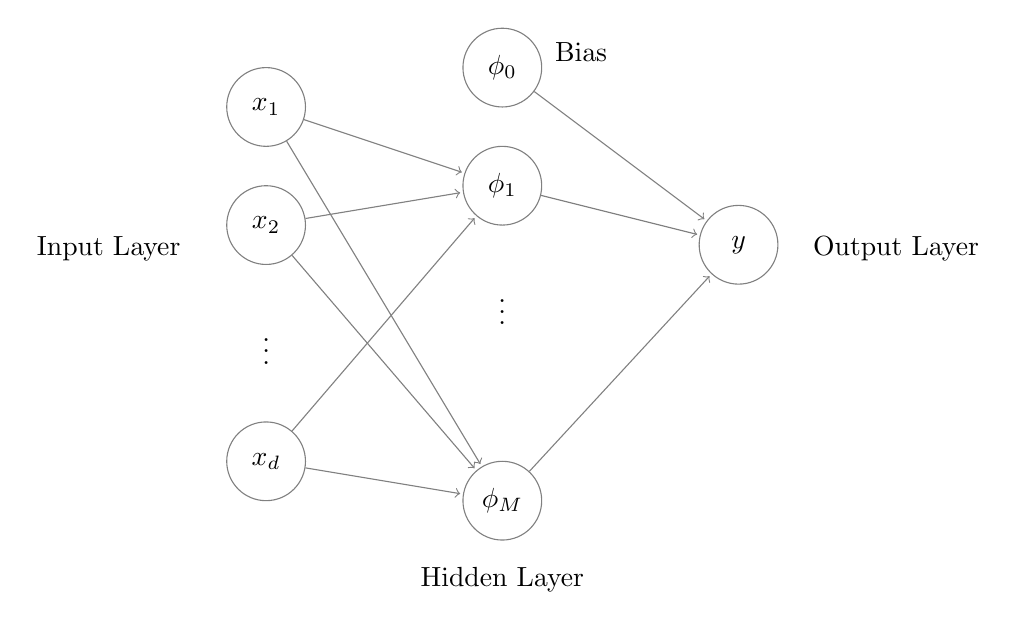
\begin{tikzpicture}[shorten >=1pt,->,draw=black!50, node distance=2cm']

        % Labels for the layers
        \node[align=center] (inputlabel) at (-2,-2.8) {Input Layer};
        \node[align=center] (hiddenlabel) at (3,-7) {Hidden Layer};
        \node[align=center] (hiddenlabel) at (4,-0.3) {Bias};
        \node[align=center] (outputlabel) at (8,-2.8) {Output Layer};

        % Input Layer Nodes
        \node[circle, draw, minimum size=1cm] (I-1) at (0,-1) {$x_1$};
        \node[circle, draw, minimum size=1cm] (I-2) at (0,-2.5) {$x_2$};
        \node[] (I-dots) at (0,-4) {$\vdots$};
        \node[circle, draw, minimum size=1cm] (I-d) at (0,-5.5) {$x_d$};
    
        % Hidden Layer Nodes
        \node[circle, draw, minimum size=1cm] (H-0) at (3,-0.5) {$\phi_0$};
        \node[circle, draw, minimum size=1cm] (H-1) at (3,-2) {$\phi_1$};
        \node[] (H-dots) at (3,-3.5) {$\vdots$};
        \node[circle, draw, minimum size=1cm] (H-M) at (3,-6) {$\phi_M$};
    
        % Output Layer Node
        \node[circle, draw, minimum size=1cm] (O) at (6,-2.75) {$y$};
    
        % Connect input layer to hidden layer (excluding phi_0)
        \foreach \i in {1,2,d}
            \foreach \j in {1,M}
                \draw[->] (I-\i) -- (H-\j);
    
        % Connect phi_0 directly to output layer
        \draw[->] (H-0) -- (O);

        % Connect other hidden layer nodes to output layer
        \foreach \j in {1,M}
            \draw[->] (H-\j) -- (O);
    
    \end{tikzpicture}
    \caption{Radial basis function neural network}
    \label{fig:rbf_nn_architecture}
\end{figure}

\subsubsection{Network Construction}

Neural networks work best with data that is specified between a specific 
range (\citeboth{mendelsohn1993}).
Also, based on the unit root tests in Table \ref{table: unitroot} the variables in the dataset $X$, described in \ref{section: prep},
only achieve stationary at first difference.
Therefore, all of the 
variables in the dataset $X$ were normalised using a z-score normalisation and differenced,
as described in Algorithm \ref{alg:z_score_differencing}. 

\begin{algorithm}[H]
    \caption{Z-Score Normalisation and Differencing of Variables}
    \label{alg:z_score_differencing}
    \KwData{Dataset $X$ with variables $X_1 = FTSE_{250}, X_2 = CPI, X_3 = EXCHG, X_4 = INT, X_5 = M3$}
    \KwResult{Normalised and differenced dataset $Z$}
    
    \For{each variable $X_i$ in $X$}{
        \textbf{Compute:} $\mu_i \leftarrow \frac{1}{m} \sum_{j=1}^{m} X_{ij}$\;
        \textbf{Compute:} $\sigma_i \leftarrow \sqrt{\frac{1}{m} \sum_{j=1}^{m} (X_{ij} - \mu_i)^2}$\;
        \For{each observation $X_{ij}$ in $X_i$}{
            \textbf{Normalise:} $Z_{ij} \leftarrow \frac{X_{ij} - \mu_i}{\sigma_i}$\;
        }
        \For{each observation $Z_{ij}$ from the second observation to the last}{
            \textbf{Difference:} $D_{ij} \leftarrow Z_{ij} - Z_{i(j-1)}$\;
        }
    }
    \textbf{Update:} $Z_i \leftarrow D_i$ \;
\end{algorithm}

The inputs into the network were 4-dimensional input vectors, \(\boldsymbol{\mathrm{x_i}}\), from the differenced, normalised dataset $Z$

\begin{align}
    \boldsymbol{\mathrm{x_i}} = \{\Delta \text{CPI}_i, \Delta \text{EXCHG}_i, \Delta \text{INT}_i, \Delta \text{M3}_i\}
\end{align}

where \(\Delta \text{CPI}_i\), \(\Delta \text{EXCHG}_i\), \(\Delta \text{INT}_i\), and \(\Delta \text{M3}_i\) 
represented differenced monthly values in the CPI, USD/GBP exchange rate, interest rate, and M3 money supply, respectively. 

The output was a one-dimensional output vector, \(\boldsymbol{\mathrm{y_i}}\) from the dataset $Z$, representing differenced monthly values in the FTSE250.


\begin{align}
    \boldsymbol{\mathrm{y_i}} = \{\Delta \text{FTSE}_{250_i}\}
\end{align}

The radial basis function neural network was programmed into Python. The Bayesian kernel regression approach outlined by 
\citeboth{bishop1995}, using the GaussianProcessRegressor package in Python was employed to model the network. For a 
detailed description of this construction please refer to the \hyperref[sec: appendix]{Appendix}.

The approach outlined in the \hyperref[sec: appendix]{Appendix} was used to conduct the train-test process:
\begin{enumerate}
    \item The optimal hyperparameters in the covariance function \eqref{eq: gimq} 
    were computed using GridSearch Cross Validation. These hyperparameters were:
    \begin{enumerate}
        \item $\alpha$: a regularisation parameter representing a small quantity
        that was added to the diagonals of the covariance matrix to ensure it was 
        invertible. 
        \item $\beta$: the power in the covariance function, which controlled the shape of the function.
        \item $\sigma$: a parameter which controlled how much of the noise in the data the kernel accounted for. It moderated the risk of overfitting and underfitting.
        \item Length scale: a parameter that controlled the influence that each kernel was to have. Analogous to 
        the width that each radial basis function neuron possesses.
    \end{enumerate}
    \item Training inputs $\boldsymbol{\mathrm{x}}_1, \boldsymbol{\mathrm{x}}_2,\ldots \boldsymbol{\mathrm{x}}_{n}$
    and corresponding outputs \( y = \{y_1, y_2, \dots, y_n\} \) were successively passed through the 
    covariance function $(x,x')$, to obtain the matrix of the pairwise covariance of 
    all training observations, $K$.
    \item A $4$-dimensional input space $X$ took in an individual training observation $(\boldsymbol{\mathrm{x}}_{i}, y_i)$ and 
    calculated the posterior weights distribution. 
    Each possible weight vector $w$ represented a different function, explicitly 
    based on the radial basis function covariance function, that could fit the data. In the 
    hidden layer the expectation of this distribution was then taken, which
    combined all the weights and found the mean, weighted by the 
    respective probabilities. This represented the best functional estimate of the price movement. Based on this estimate 
    the predicted output was generated.
    \item The testing process was conducted similarly. The 
    posterior weight distribution that contained the information of the training phase became the new 
    prior distribution. From this the posterior weight distributions for the test observations \eqref{eq: testw}
    were calculated, and then the predictive output was found (\citeboth{rasmussen2006}).
    
    \begin{align}
        p(y_{*}|x_{*}, X, y) = \mathcal{N}(\sigma_{n}^{2} x_{*}^{T}A^{-1}Xy, x_{*}^{T}A^{-1}x_{*}) \label{eq: testw}
    \end{align}
\end{enumerate}

A short-term and long-term forecast was conducted using this process. For the short-term forecast a test set of 5 months was used, and for the long-term forecast a test set of 57 months was used.


\section{Results}
\label{sec: results}

\subsection{ARDL-ECM}

\begin{table}[h!]
    \centering
    \label{table: unitroot}
    \caption{Augmented Dickey-Fuller (ADF) Unit Root Test\tablefootnote{All of the variables are tested in natural logarithmic form. The asterisks *, **, ***, and **** denote statistical significance
    at the 1$\%$, 2.5$\%$, 5$\%$ and 10$\%$ significance levels.}}
    \begin{tabular}{lccc}
        \toprule
        \textbf{Variable} & \textbf{Level ADF} & \textbf{First Difference ADF} & \textbf{Stationarity} \\
        \midrule
        FTSE$_{250}$ & $-3.2646^{****}$ & $-6.6892^{*}$ & At first difference \\
        CPI          & $-1.4594$ & $-4.705^{*}$ & At first difference \\
        EXCHG        & $-2.2467$ & $-7.3855^{*}$ & At first difference \\
        INT          & $-2.0946$ & $-4.1156^{*}$ & At first difference \\
        M3           & $-0.70827$ & $-6.3806^{*}$ & At first difference \\
        \bottomrule
    \end{tabular}
\end{table}


The optimum lags for the ARDL model were ($FTSE_{250} = 5$, $CPI = 4$, $EXCHG=7$, $INT =7$, $M3=4$). The resulting F-statistic of $4.1$ was compared against the critical values
given by \citeboth{pesaran2001}, providing evidence of cointegration 
at the $10\%$, $5\%$ and $2.5\%$ significance levels, but not at the $1\%$ 
level.

\begin{table}[h!]
    \centering
    \caption{ARDL Bounds Test Critical Values}
    \begin{tabular}{lcccc}
        \toprule
        \textbf{Order} & \textbf{10$\%$} & \textbf{5$\%$} & \textbf{2.5$\%$} & \textbf{1$\%$} \\
        \midrule
        I(0) & $2.20$ & $2.56$ & $2.88$ & $3.29$ \\
        I(1) & $3.09$ & $3.49$ & $3.87$  & $4.37$ \\
        \bottomrule
    \end{tabular}
\end{table}

\begin{table}[h!]
    \centering
    \caption{Coefficients Estimates}
    \begin{tabular}{llll}
        \toprule
        \textbf{Variable} & \textbf{Long-Run Coefficient} & \textbf{Variable} & \textbf{Short-Run Coefficient} \\
        \midrule
        FTSE$_{250}$ & $-$ & FTSE$_{250}$ $(-5)$  & $-0.033089$ \\
        CPI & $3.157179$ & CPI $(-4)$ & $-0.921235$ \\
        INT & $-0.1341097^{***}$ & INT $(-7)$ & $-0.034572^{****}$\\
        EXCHG &  $-0.890146^{****}$ & EXCHG $(-7)$ & $0.122318$ \\
        M3 & $-0.1141114$ & M3 $(-4)$ & $-0.527798^{***}$ \\
        Intercept & $-3.447767$ & ECT $(-1)$ & $-0.1794^{**}$ \\
        \bottomrule
    \end{tabular}
\end{table}

\begin{table}[h!]
    \centering
    \caption{Diagnostic Tests}
    \begin{tabular}{llll}
        \toprule
        \textbf{Condition} & \textbf{Test} & \textbf{p-value} & \textbf{Result} \\
        \midrule
        Autocorrelation & Box-Ljung Test & $0.9926$ & No autocorrelation \\
        Heteroskedascity & Breusch-Pagan Test & $0.3635$ & Homoskedascity \\
        Normality & Shapiro-Wilk Test & $3.889$e-$08$ & Normality \\
        CUSUM & CUSUM Test & $-$ & Stable \\
        CUSUM$^2$ & CUSUM$^2$ Test & $-$ & Stable \\
        \bottomrule
    \end{tabular}
\end{table}

\subsubsection{Short-term Impacts}

The interest rate had a significantly
negative short-term impact on the FTSE250 price in the short term. 
This can be attributed to the immediate effect of interest rate hikes, 
which decrease the present value of future earnings according to the 
Discounted Cash Flow (DCF) valuation model, thereby 
affecting investor sentiment and depressing stock prices. 
This finding was consistent with the studies by 
\citeboth{alam2009}, \citeboth{demir2019}, and \citeboth{neifar2023}.

The money supply had a significantly negative short-term effect on the 
FTSE250 price, as noted by \citeboth{olawale2014}. 
According to \citeboth{sellin2001}, this aligned with the Keynesian argument 
that an increase in money supply leads to expectations of a future 
monetary contraction. This expectation increases the demand for 
funds, driving up current interest rates and reducing stock prices 
through the same mechanism as described previously.

In the short-term, before structural shifts can materialise, the
weakening of the Pound against the Dollar had a positive, but 
insignificant effect. As the USD has been 
the global reserve currency for many decades, the depreciation of the Pound 
against it would lead to increased revenue in Pound terms for FTSE250 
companies with substantial overseas operations. 
This is because their foreign earnings, 
when converted back into Pounds, will be worth more, 
potentially increasing profits. However, the insignificant impact suggests 
that FTSE250 firms are resilient to short-term fluctuations in the stock market 
price. The possible reasons for this are that they have diversified 
operations, meaning fluctuations against the Dollar will not threaten 
their profits and they use hedging strategies involving financial instruments 
such as currency forwards which protect against volatility. 

The insignificance of inflation, defined as a positive 
increase in the CPI, confirmed the findings of 
\citeboth{gultekin1983}, \citeboth{firth1979} and \citeboth{neifar2023}. 
The CPI as a measure does not uniformly represent all sectors of the economy, 
and may consequently be unrepresentative of inflationary changes in the 
sectors that predominate the FTSE250. In addition, different sectors 
are more vulnerable to inflation than others which may distort the effect 
of inflation even further. Moreover, inflation may be anticipated 
by investors and already be factored into stock prices.

The error correction term 
was negative and statistically significant ensuring that long-run equilibrium 
can be achieved. The adjustment speed of $0.1794$ indicated that 
roughly $18\%$ of the fluctuation in the previous month's price caused by the 
macroeconomic variable movements was adjusted back to the long-run equilibrium in the subsequent month. This implies 
that it takes approximately 6 months for the FTSE250 to return to its long-run equilibrium following 
changes in the selected macroeconomic variables.

\subsubsection{Long-term Impacts}

The CPI did not have a significant effect on the FTSE250 price over the 
long-run, lending support to the findings of 
\citeboth{gultekin1983} and \citeboth{firth1979}
that the Fisher hypothesis is valid for the UK. One of the 
reasons for this may be that, since stock prices represent the 
discounted value of future cash flows (which are real), 
they are not directly impacted by inflation in the long run. Moreover, 
firms are able to pass on nominal costs to consumers which reduces
the impact of inflation.
The freer role of the Bank of England in setting monetary policy could be 
another factor in this, as a stricter monetary policy would keep inflation
in check and obscure any long-term equilibrium relationship. 

The insignificant long-term effect of the money supply can be explained by several factors.
Firstly, as discussed in \citeboth{sellin2001}, it is possible that the FTSE250 is efficient in processing changes in the 
money supply, at least over certain intervals if not always. This would mean anticipated changes in the money supply would not affect the stock market price, only the
unanticipated component of a change in money supply would, as established by \citeboth{sorensen1982} and \citeboth{bernanke2005}. 
It is also possible that the M3 measure is too broad of a measure and includes overly illiquid components that are not as impactful 
on the stock market dynamics. 

The USD/GBP exchange rate significantly positively impacted the FTSE250 price, confirming the findings of 
\citeboth{wong2022}. That there is a significant relationship is not surprising, because whilst the FTSE250 is a more domestic indicator of the London Stock Exchange than the FTSE 100 Index, 
at times nearly $50\%$ of its earnings have come from abroad, indicating that 
the value of the Pound has a significant impact on this stock market. There are many reasons for why this effect is observed.
In the long run, the appreciation of the Pound would decrease the 
cost of imports, thereby increasing the 
profits of FTSE250 companies and inflating their share prices.
Moreover, a stronger Pound makes UK assets more appealing to foreign investors, as their investments would be worth more when converted back to their domestic currencies.
This would drive up demand for UK stocks and positively influence the 
FTSE250 price.

The interest rate was also found to have significant negative long-term and short-term effects on the stock market, confirming the findings of \citeboth{alam2009}, \citeboth{demir2019} and \citeboth{neifar2023}
This can be explained by the fact that higher interest 
rates increase the cost of borrowing for companies, leading to reduced investment 
and lower future earnings potential, in turn depressing stock prices. 
Furthermore, as per the flight-to-quality phenomenon, persistently higher interest rates make bonds and other fixed-income 
investments more attractive relative to stocks, leading investors to shift 
their portfolios away from equities and toward safer assets over time (\citeboth{asgharian2016}). 
In the short term, interest rate hikes immediately decrease the present value of earnings, as per the 
DCF valuation model, and depress prices.




\subsection{RBFNN}

\subsubsection{Short-term Forecast}


The short-term prediction yielded MAE = $0.07$ and 
$R^2 = 61\%$ for a 5-month time horizon. The results obtained are presented in Figure \ref{fig:shortmonthly}.
The significantly better performance of the model in the short-run
indicates that the selected macroeconomic variables possess
a stronger predictive power over shorter periods. This was highlighted 
earlier in the ARDL model, with the interest rate and money supply significantly
impacting the FTSE250 price in the short-run.



\begin{figure}[H]
    \centering
    \hspace*{-1.5cm}
    % Created by tikzDevice version 0.12.6 on 2024-08-15 14:40:36
% !TEX encoding = UTF-8 Unicode
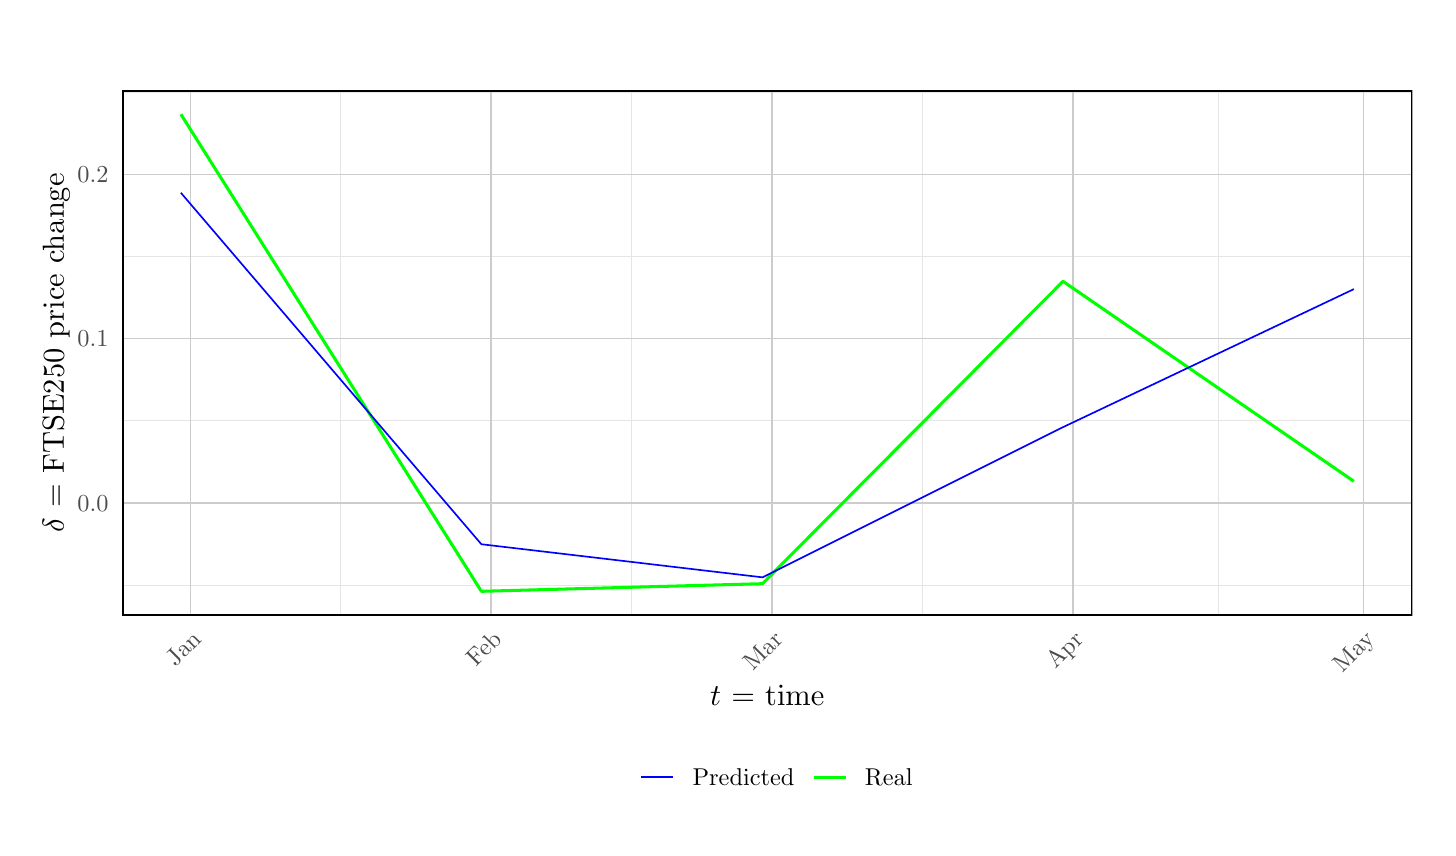
\begin{tikzpicture}[x=1pt,y=1pt]
\definecolor{fillColor}{RGB}{255,255,255}
\path[use as bounding box,fill=fillColor,fill opacity=0.00] (0,0) rectangle (505.89,289.08);
\begin{scope}
\path[clip] ( 34.16, 76.79) rectangle (500.39,266.42);
\definecolor{drawColor}{gray}{0.90}

\path[draw=drawColor,line width= 0.3pt,line join=round] ( 34.16, 87.71) --
	(500.39, 87.71);

\path[draw=drawColor,line width= 0.3pt,line join=round] ( 34.16,147.06) --
	(500.39,147.06);

\path[draw=drawColor,line width= 0.3pt,line join=round] ( 34.16,206.41) --
	(500.39,206.41);

\path[draw=drawColor,line width= 0.3pt,line join=round] ( 34.16,265.76) --
	(500.39,265.76);

\path[draw=drawColor,line width= 0.3pt,line join=round] (113.15, 76.79) --
	(113.15,266.42);

\path[draw=drawColor,line width= 0.3pt,line join=round] (218.23, 76.79) --
	(218.23,266.42);

\path[draw=drawColor,line width= 0.3pt,line join=round] (323.32, 76.79) --
	(323.32,266.42);

\path[draw=drawColor,line width= 0.3pt,line join=round] (430.16, 76.79) --
	(430.16,266.42);
\definecolor{drawColor}{gray}{0.80}

\path[draw=drawColor,line width= 0.6pt,line join=round] ( 34.16,117.38) --
	(500.39,117.38);

\path[draw=drawColor,line width= 0.6pt,line join=round] ( 34.16,176.73) --
	(500.39,176.73);

\path[draw=drawColor,line width= 0.6pt,line join=round] ( 34.16,236.08) --
	(500.39,236.08);

\path[draw=drawColor,line width= 0.6pt,line join=round] ( 58.85, 76.79) --
	( 58.85,266.42);

\path[draw=drawColor,line width= 0.6pt,line join=round] (167.44, 76.79) --
	(167.44,266.42);

\path[draw=drawColor,line width= 0.6pt,line join=round] (269.02, 76.79) --
	(269.02,266.42);

\path[draw=drawColor,line width= 0.6pt,line join=round] (377.61, 76.79) --
	(377.61,266.42);

\path[draw=drawColor,line width= 0.6pt,line join=round] (482.70, 76.79) --
	(482.70,266.42);
\definecolor{drawColor}{RGB}{0,255,0}

\path[draw=drawColor,line width= 1.1pt,line join=round] ( 55.35,257.80) --
	(163.94, 85.41) --
	(265.52, 88.16) --
	(374.11,197.41) --
	(479.20,125.17);
\definecolor{drawColor}{RGB}{0,0,255}

\path[draw=drawColor,line width= 0.6pt,line join=round] ( 55.35,229.43) --
	(163.94,102.42) --
	(265.52, 90.46) --
	(374.11,144.72) --
	(479.20,194.60);
\definecolor{drawColor}{RGB}{0,0,0}

\path[draw=drawColor,line width= 1.1pt,line join=round,line cap=round] ( 34.16, 76.79) rectangle (500.39,266.42);
\end{scope}
\begin{scope}
\path[clip] (  0.00,  0.00) rectangle (505.89,289.08);
\definecolor{drawColor}{gray}{0.30}

\node[text=drawColor,anchor=base east,inner sep=0pt, outer sep=0pt, scale=  0.88] at ( 29.21,114.35) {0.0};

\node[text=drawColor,anchor=base east,inner sep=0pt, outer sep=0pt, scale=  0.88] at ( 29.21,173.70) {0.1};

\node[text=drawColor,anchor=base east,inner sep=0pt, outer sep=0pt, scale=  0.88] at ( 29.21,233.05) {0.2};
\end{scope}
\begin{scope}
\path[clip] (  0.00,  0.00) rectangle (505.89,289.08);
\definecolor{drawColor}{gray}{0.30}

\node[text=drawColor,rotate= 45.00,anchor=base east,inner sep=0pt, outer sep=0pt, scale=  0.88] at ( 63.14, 67.55) {Jan};

\node[text=drawColor,rotate= 45.00,anchor=base east,inner sep=0pt, outer sep=0pt, scale=  0.88] at (171.73, 67.55) {Feb};

\node[text=drawColor,rotate= 45.00,anchor=base east,inner sep=0pt, outer sep=0pt, scale=  0.88] at (273.31, 67.55) {Mar};

\node[text=drawColor,rotate= 45.00,anchor=base east,inner sep=0pt, outer sep=0pt, scale=  0.88] at (381.90, 67.55) {Apr};

\node[text=drawColor,rotate= 45.00,anchor=base east,inner sep=0pt, outer sep=0pt, scale=  0.88] at (486.99, 67.55) {May};
\end{scope}
\begin{scope}
\path[clip] (  0.00,  0.00) rectangle (505.89,289.08);
\definecolor{drawColor}{RGB}{0,0,0}

\node[text=drawColor,anchor=base,inner sep=0pt, outer sep=0pt, scale=  1.10] at (267.27, 44.09) {$t$ = time};
\end{scope}
\begin{scope}
\path[clip] (  0.00,  0.00) rectangle (505.89,289.08);
\definecolor{drawColor}{RGB}{0,0,0}

\node[text=drawColor,rotate= 90.00,anchor=base,inner sep=0pt, outer sep=0pt, scale=  1.10] at ( 13.08,171.61) {$\delta$ = FTSE250 price change};
\end{scope}
\begin{scope}
\path[clip] (  0.00,  0.00) rectangle (505.89,289.08);
\definecolor{drawColor}{RGB}{0,0,255}

\path[draw=drawColor,line width= 0.6pt,line join=round] (221.75, 18.23) -- (233.31, 18.23);
\end{scope}
\begin{scope}
\path[clip] (  0.00,  0.00) rectangle (505.89,289.08);
\definecolor{drawColor}{RGB}{0,255,0}

\path[draw=drawColor,line width= 1.1pt,line join=round] (284.01, 18.23) -- (295.57, 18.23);
\end{scope}
\begin{scope}
\path[clip] (  0.00,  0.00) rectangle (505.89,289.08);
\definecolor{drawColor}{RGB}{0,0,0}

\node[text=drawColor,anchor=base west,inner sep=0pt, outer sep=0pt, scale=  0.88] at (240.26, 15.20) {Predicted};
\end{scope}
\begin{scope}
\path[clip] (  0.00,  0.00) rectangle (505.89,289.08);
\definecolor{drawColor}{RGB}{0,0,0}

\node[text=drawColor,anchor=base west,inner sep=0pt, outer sep=0pt, scale=  0.88] at (302.51, 15.20) {Real};
\end{scope}
\end{tikzpicture}
  
    \caption{Short-term predicted vs real monthly FTSE250 changes}
    \label{fig:shortmonthly}
\end{figure}



In the short-term the market movements
are more closely tied to recent deviations in the economy. This is because,
theoretically, 
the short-run is not exposed to the various unforeseen external shocks and structural changes
that dilute the relationship between these variables and the stock market in the 
long-run. As the prediction window expands in regression problems, 
more uncertainty and unknowns are introduced, which translates into 
lower predictive quality. Furthermore, as the time horizon extends into the long-run, fundamental factors 
begin to matter a lot more. The compound effect of earnings, cash flows,
innovations and managerial efficiencies begins to outweigh the 
influence of fluctuating macroeconomic variables. Essentially, firms become accustomed 
to the changed economic environment and over time. Thus, in the short-run 
a different phenomenon is observed.



\subsubsection{Long-term Forecast}
The model returned a mean absolute error of MAE $=0.16$ and 
$R^2 = 9\%$ for the long-term prediction, providing a 
$2.4\%$ increase in the $R^2$ obtained by the ARDL-ECM model. The results are presented 
in Figure \ref{fig:longmonthly}.

The interpretation of this is that, over the long-run (4-5 years), the variations in the 
Consumer Price Index, interest rate, USD/GBP exchange rate, and M3 money 
supply explain or account for $9\%$ of the fluctuations of the
monthly FTSE250 value. This relates closely to the findings of \citeboth{conover1999}, 
who used an econometric model to establish that $4\%$ of the variation in monthly UK stock returns can be 
explained by variations in the money supply. It also suggests a higher level of influence 
than the ARDL-ECM model provided, that only $R^2=3.4\%$ of the monthly FTSE250 variations 
are affected by the selected macroeconomic variables, demonstrating the ability of machine learning
methods to capture subtle patterns in the data unavailable to econometric models. 

\begin{figure}[H]
    \centering
    \hspace*{-1.5cm}
    % Created by tikzDevice version 0.12.6 on 2024-08-15 14:44:41
% !TEX encoding = UTF-8 Unicode
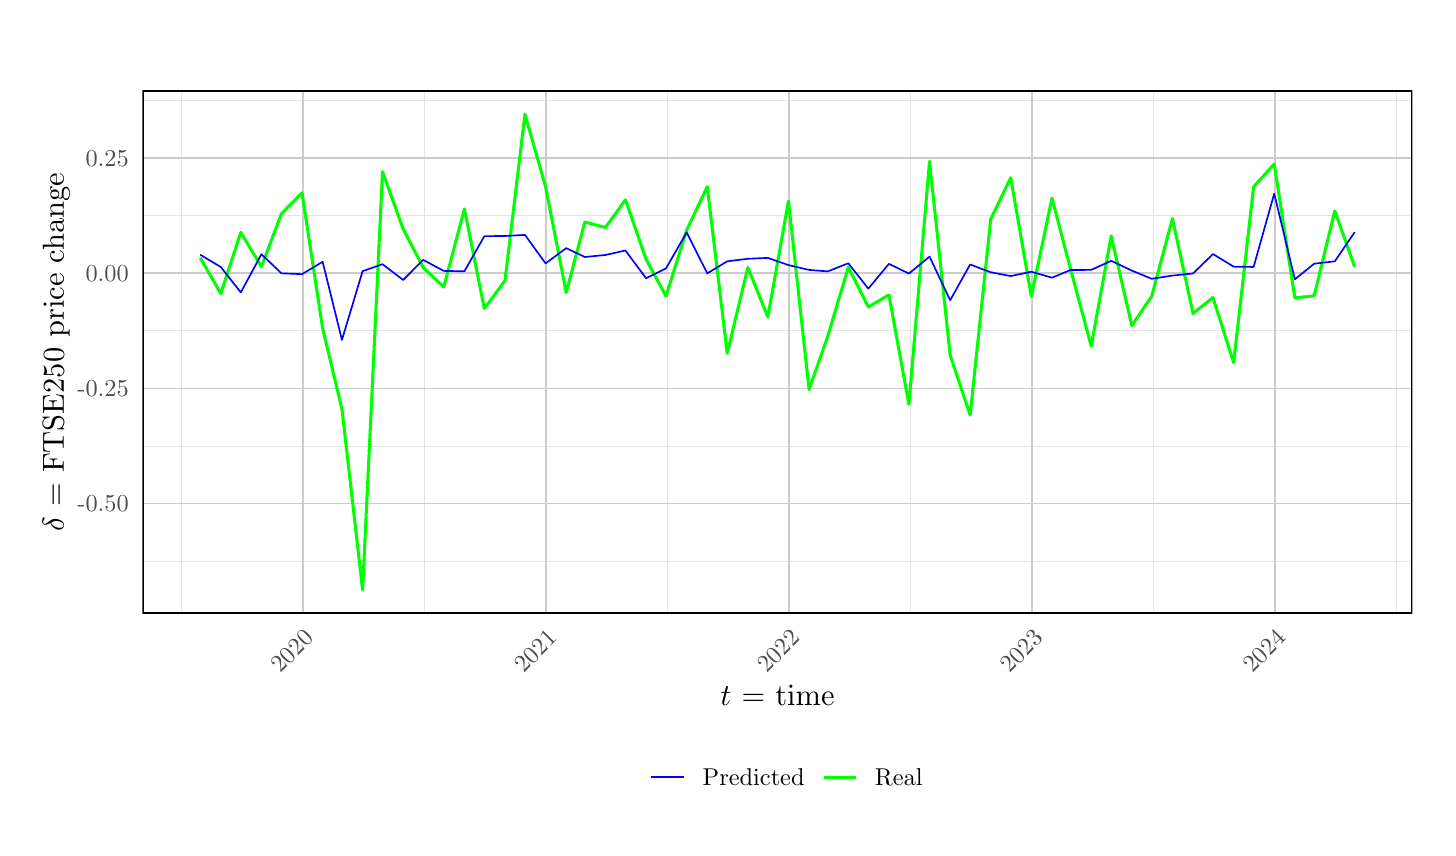
\begin{tikzpicture}[x=1pt,y=1pt]
\definecolor{fillColor}{RGB}{255,255,255}
\path[use as bounding box,fill=fillColor,fill opacity=0.00] (0,0) rectangle (505.89,289.08);
\begin{scope}
\path[clip] ( 41.49, 77.31) rectangle (500.39,266.42);
\definecolor{drawColor}{gray}{0.90}

\path[draw=drawColor,line width= 0.3pt,line join=round] ( 41.49, 96.28) --
	(500.39, 96.28);

\path[draw=drawColor,line width= 0.3pt,line join=round] ( 41.49,137.92) --
	(500.39,137.92);

\path[draw=drawColor,line width= 0.3pt,line join=round] ( 41.49,179.57) --
	(500.39,179.57);

\path[draw=drawColor,line width= 0.3pt,line join=round] ( 41.49,221.21) --
	(500.39,221.21);

\path[draw=drawColor,line width= 0.3pt,line join=round] ( 41.49,262.86) --
	(500.39,262.86);

\path[draw=drawColor,line width= 0.3pt,line join=round] ( 55.49, 77.31) --
	( 55.49,266.42);

\path[draw=drawColor,line width= 0.3pt,line join=round] (143.38, 77.31) --
	(143.38,266.42);

\path[draw=drawColor,line width= 0.3pt,line join=round] (231.26, 77.31) --
	(231.26,266.42);

\path[draw=drawColor,line width= 0.3pt,line join=round] (319.03, 77.31) --
	(319.03,266.42);

\path[draw=drawColor,line width= 0.3pt,line join=round] (406.79, 77.31) --
	(406.79,266.42);

\path[draw=drawColor,line width= 0.3pt,line join=round] (494.68, 77.31) --
	(494.68,266.42);
\definecolor{drawColor}{gray}{0.80}

\path[draw=drawColor,line width= 0.6pt,line join=round] ( 41.49,117.10) --
	(500.39,117.10);

\path[draw=drawColor,line width= 0.6pt,line join=round] ( 41.49,158.75) --
	(500.39,158.75);

\path[draw=drawColor,line width= 0.6pt,line join=round] ( 41.49,200.39) --
	(500.39,200.39);

\path[draw=drawColor,line width= 0.6pt,line join=round] ( 41.49,242.04) --
	(500.39,242.04);

\path[draw=drawColor,line width= 0.6pt,line join=round] ( 99.38, 77.31) --
	( 99.38,266.42);

\path[draw=drawColor,line width= 0.6pt,line join=round] (187.38, 77.31) --
	(187.38,266.42);

\path[draw=drawColor,line width= 0.6pt,line join=round] (275.15, 77.31) --
	(275.15,266.42);

\path[draw=drawColor,line width= 0.6pt,line join=round] (362.91, 77.31) --
	(362.91,266.42);

\path[draw=drawColor,line width= 0.6pt,line join=round] (450.68, 77.31) --
	(450.68,266.42);
\definecolor{drawColor}{RGB}{0,255,0}

\path[draw=drawColor,line width= 1.1pt,line join=round] ( 62.35,205.92) --
	( 69.80,193.01) --
	( 77.01,215.09) --
	( 84.47,202.69) --
	( 91.68,221.81) --
	( 99.14,229.38) --
	(106.59,180.36) --
	(113.56,151.33) --
	(121.02, 85.90) --
	(128.23,237.03) --
	(135.68,216.32) --
	(142.90,202.45) --
	(150.35,195.34) --
	(157.81,223.55) --
	(165.02,187.59) --
	(172.47,197.66) --
	(179.69,257.83) --
	(187.14,231.57) --
	(194.60,193.36) --
	(201.33,218.85) --
	(208.78,216.86) --
	(216.00,226.88) --
	(223.45,205.44) --
	(230.66,192.06) --
	(238.12,215.90) --
	(245.57,231.61) --
	(252.78,171.41) --
	(260.24,202.43) --
	(267.45,184.51) --
	(274.91,226.41) --
	(282.36,158.32) --
	(289.09,177.51) --
	(296.55,202.53) --
	(303.76,188.17) --
	(311.21,192.52) --
	(318.43,152.99) --
	(325.88,240.78) --
	(333.34,170.75) --
	(340.55,149.09) --
	(348.00,219.92) --
	(355.22,234.86) --
	(362.67,191.99) --
	(370.13,227.47) --
	(376.86,201.74) --
	(384.31,174.00) --
	(391.53,213.84) --
	(398.98,181.39) --
	(406.19,192.11) --
	(413.65,220.07) --
	(421.10,185.83) --
	(428.31,191.56) --
	(435.77,168.01) --
	(442.98,231.53) --
	(450.44,239.81) --
	(457.89,191.42) --
	(464.86,192.19) --
	(472.32,222.85) --
	(479.53,202.58);
\definecolor{drawColor}{RGB}{0,0,255}

\path[draw=drawColor,line width= 0.6pt,line join=round] ( 62.35,207.04) --
	( 69.80,202.58) --
	( 77.01,193.41) --
	( 84.47,207.21) --
	( 91.68,200.32) --
	( 99.14,200.01) --
	(106.59,204.48) --
	(113.56,176.23) --
	(121.02,201.09) --
	(128.23,203.61) --
	(135.68,197.91) --
	(142.90,205.17) --
	(150.35,201.19) --
	(157.81,201.04) --
	(165.02,213.74) --
	(172.47,213.80) --
	(179.69,214.20) --
	(187.14,203.90) --
	(194.60,209.41) --
	(201.33,206.21) --
	(208.78,206.94) --
	(216.00,208.57) --
	(223.45,198.53) --
	(230.66,202.09) --
	(238.12,215.10) --
	(245.57,200.30) --
	(252.78,204.65) --
	(260.24,205.57) --
	(267.45,205.89) --
	(274.91,203.29) --
	(282.36,201.54) --
	(289.09,201.01) --
	(296.55,203.94) --
	(303.76,194.77) --
	(311.21,203.74) --
	(318.43,200.22) --
	(325.88,206.35) --
	(333.34,190.58) --
	(340.55,203.50) --
	(348.00,200.70) --
	(355.22,199.32) --
	(362.67,200.88) --
	(370.13,198.74) --
	(376.86,201.52) --
	(384.31,201.55) --
	(391.53,204.83) --
	(398.98,201.30) --
	(406.19,198.34) --
	(413.65,199.50) --
	(421.10,200.25) --
	(428.31,207.28) --
	(435.77,202.72) --
	(442.98,202.61) --
	(450.44,229.12) --
	(457.89,198.15) --
	(464.86,203.79) --
	(472.32,204.65) --
	(479.53,215.21);
\definecolor{drawColor}{RGB}{0,0,0}

\path[draw=drawColor,line width= 1.1pt,line join=round,line cap=round] ( 41.49, 77.31) rectangle (500.39,266.42);
\end{scope}
\begin{scope}
\path[clip] (  0.00,  0.00) rectangle (505.89,289.08);
\definecolor{drawColor}{gray}{0.30}

\node[text=drawColor,anchor=base east,inner sep=0pt, outer sep=0pt, scale=  0.88] at ( 36.54,114.07) {-0.50};

\node[text=drawColor,anchor=base east,inner sep=0pt, outer sep=0pt, scale=  0.88] at ( 36.54,155.72) {-0.25};

\node[text=drawColor,anchor=base east,inner sep=0pt, outer sep=0pt, scale=  0.88] at ( 36.54,197.36) {0.00};

\node[text=drawColor,anchor=base east,inner sep=0pt, outer sep=0pt, scale=  0.88] at ( 36.54,239.01) {0.25};
\end{scope}
\begin{scope}
\path[clip] (  0.00,  0.00) rectangle (505.89,289.08);
\definecolor{drawColor}{gray}{0.30}

\node[text=drawColor,rotate= 45.00,anchor=base east,inner sep=0pt, outer sep=0pt, scale=  0.88] at (103.66, 68.07) {2020};

\node[text=drawColor,rotate= 45.00,anchor=base east,inner sep=0pt, outer sep=0pt, scale=  0.88] at (191.67, 68.07) {2021};

\node[text=drawColor,rotate= 45.00,anchor=base east,inner sep=0pt, outer sep=0pt, scale=  0.88] at (279.43, 68.07) {2022};

\node[text=drawColor,rotate= 45.00,anchor=base east,inner sep=0pt, outer sep=0pt, scale=  0.88] at (367.20, 68.07) {2023};

\node[text=drawColor,rotate= 45.00,anchor=base east,inner sep=0pt, outer sep=0pt, scale=  0.88] at (454.96, 68.07) {2024};
\end{scope}
\begin{scope}
\path[clip] (  0.00,  0.00) rectangle (505.89,289.08);
\definecolor{drawColor}{RGB}{0,0,0}

\node[text=drawColor,anchor=base,inner sep=0pt, outer sep=0pt, scale=  1.10] at (270.94, 44.09) {$t$ = time};
\end{scope}
\begin{scope}
\path[clip] (  0.00,  0.00) rectangle (505.89,289.08);
\definecolor{drawColor}{RGB}{0,0,0}

\node[text=drawColor,rotate= 90.00,anchor=base,inner sep=0pt, outer sep=0pt, scale=  1.10] at ( 13.08,171.86) {$\delta$ = FTSE250 price change};
\end{scope}
\begin{scope}
\path[clip] (  0.00,  0.00) rectangle (505.89,289.08);
\definecolor{drawColor}{RGB}{0,0,255}

\path[draw=drawColor,line width= 0.6pt,line join=round] (225.41, 18.23) -- (236.98, 18.23);
\end{scope}
\begin{scope}
\path[clip] (  0.00,  0.00) rectangle (505.89,289.08);
\definecolor{drawColor}{RGB}{0,255,0}

\path[draw=drawColor,line width= 1.1pt,line join=round] (287.67, 18.23) -- (299.24, 18.23);
\end{scope}
\begin{scope}
\path[clip] (  0.00,  0.00) rectangle (505.89,289.08);
\definecolor{drawColor}{RGB}{0,0,0}

\node[text=drawColor,anchor=base west,inner sep=0pt, outer sep=0pt, scale=  0.88] at (243.92, 15.20) {Predicted};
\end{scope}
\begin{scope}
\path[clip] (  0.00,  0.00) rectangle (505.89,289.08);
\definecolor{drawColor}{RGB}{0,0,0}

\node[text=drawColor,anchor=base west,inner sep=0pt, outer sep=0pt, scale=  0.88] at (306.18, 15.20) {Real};
\end{scope}
\end{tikzpicture}
  
    \caption{Long-term predicted vs real monthly FTSE250 changes}
    \label{fig:longmonthly}
\end{figure}



In the context of a phenomenon as complex as the stock market,
which is influenced by an inumerable quantity of factors such as investor sentiment
- inherently irrational, 
political instability, geopolitical shocks, corporate governance, and financial regulation, this result 
unsurprising. Furthermore, the selection of economic variables in this study
is by no means exhaustive; commodity prices, international trade dynamics,
economic growth, and many other variables also exert a non-insignificant 
effect on the stock market.


\section{Conclusion}
\label{sec: conc}


Stock markets provide important information on the economy, 
and economic policymakers are vigilant in tracking the fluctuations 
in these markets, and try to forecast the 
forthcoming fluctuations based on policy changes that affect the macroeconomy.
Within this context, the study examined the 
impacts of the interest rate, USD/GBP
exchange rate, the Consumer Price Index, and 
M3 money supply market activity on
the FTSE250 over the October 1993 – April 2024 period.
The results suggested a cointegrated long-run
relationship between the macroeconomic variables and the stock market index. 
The long-run coefficients implied that
increases in the interest rate and depreciation in the exchange rate
significantly depress the FTSE250 value. 
Policymakers dealing with forecasting the UK stock markets
should consider the factors in the study, and to raise the stock
market's value, a lower interest rate regime should be adopted. This will 
stimulate consumer activity, reduce operating costs for firms, and make 
stocks more attractive investments, thereby increasing the stock market value. 
In addition, the Pound should be increased in value to lower import costs 
and increase the real value of firm earnings, both of which should drive up 
the value of the stock market. The combined effect of these changes will 
create a more stimulating business environment by increasing the capital 
available to firms for research and development, and more efficient 
capital and labour, in turn 
driving economic growth and prosperity. However, 
as with all economic policy shifts, these changes may have 
unintended consequences on other areas of the economy, potentially 
undermining any positive changes. Any policy changes must cautiously be made 
with this at the forefront.


The study also investigated the efficacy of machine learning methods in 
the field of stock-econometric forecasting. The radial basis function network performed well in
short-term forecasting of the FTSE250, and offers investors with an accurate forecasting tool, 
to leverage in their trading strategies. The long-term forecast was able to improve on the ARDL-ECM model, and provides 
economists with a tool to compute non-econometric, quantitative measures of the 
long-term influence of macroeconomic variables on the stock market. 

Further research should endeavour to include other macroeconomic variables such as 
foreign direct and portfolio investment, commodity prices and economic growth.
An autoregressive neural network could also be tried, including the past values of the 
FTSE250 in the input space to provide a more accurate model. In addition, 
a more granular data set could be utilised by applying a 
Brownian bridge algorithm to generate daily macroeconomic data. This would allow 
the testing of the radial basis function neural network against other neural networks 
such as the LSTM. Other machine learning methods suited for 
forecasting such as Gradient Boosting Machines could 
also be investigated in future work in this problem domain. 

\section{Appendix}
\label{sec: appendix}


The GaussianProcessRegressor function in Python's Scikit library is based on the 
standard function

\begin{align} 
    f(x) = x^{T}w, \quad{y = f(x) + \varepsilon}
\end{align}

where $y$ differs from the function values $f(x)$ by noise which is assumed
to follow an iid Gaussian distribution 
$\mathcal{N}_1$ (\citeboth{rasmussen2006}).
\begin{align*}
    \varepsilon \sim \mathcal{N}_1 \bigl(0, \sigma_{n}^2\bigr)
\end{align*}
This assumption together with the model produces the 
probability density of the observations given the inputs, 
which is factored over cases in the training set. This is
permissible because of the independence assumption (\citeboth{rasmussen2006}).

\begin{align}
    p(y|X,w) = \prod_{i=1}^{n} p(y_i|x_i ,w) = \mathcal{N}\bigl(X^T, \sigma_{n}^2 I\bigr)
\end{align}

The weights \( w \) represent the parameters that define the relationship between the inputs and outputs. 
They are treated as random variables defined by the Gaussian distribution \eqref{eq: weight}.


A covariance function or kernel
is specified according to the characteristics of the data. In this study the
generalised inverse multiquadric is used.

\begin{align}
    k(x,x') = \biggl( ||x-x'|| + \sigma^2\biggr)^{-\beta} \label{eq: gimq}
\end{align}
and used to construct the covariance matrix $K$, which along with 
a mean function $m(x)$ forms the distribution of the the weights 

\begin{align}
    w \sim \mathcal{N}\bigl(m(x), K\bigr) \label{eq: weight}
\end{align}


The mean function $m(x)$ acts as a bias, 
providing a baseline expectation of the function values. 
This forms the prior distribution over the weights \eqref{eq: weight}.

Then, by Bayes' Theorem, 

\begin{align}
    p(w|y, X) = \frac{p(y|X,w) p(w)}{p(y|X)} \label{eq: post}
\end{align}
Using this, the posterior distribution \eqref{eq:nine} is obtained (\citeboth{rasmussen2006}).

\begin{align}
    p(w|y, X) \sim \mathcal{N}\bigl(\frac{A^{-1}Xy}{\sigma_{n}^{2}}, A^{-1}\bigr) \label{eq:nine}
\end{align}

The covariance matrix $A^{-1} = K^{-1} + \sigma_{n}^{-2}(XX^T$).
All possible $w$, weighted by their probability, are then averaged to obtain the
most likely functional estimate of the output (\citeboth{rasmussen2006}).

\bibliographystyle{plainnat}
\bibliography{paper}

\end{document}